% Options for packages loaded elsewhere
\PassOptionsToPackage{unicode}{hyperref}
\PassOptionsToPackage{hyphens}{url}
%
\documentclass[
  12pt,
]{article}
\usepackage{amsmath,amssymb}
\usepackage{lmodern}
\usepackage{setspace}
\usepackage{ifxetex,ifluatex}
\ifnum 0\ifxetex 1\fi\ifluatex 1\fi=0 % if pdftex
  \usepackage[T1]{fontenc}
  \usepackage[utf8]{inputenc}
  \usepackage{textcomp} % provide euro and other symbols
\else % if luatex or xetex
  \usepackage{unicode-math}
  \defaultfontfeatures{Scale=MatchLowercase}
  \defaultfontfeatures[\rmfamily]{Ligatures=TeX,Scale=1}
\fi
% Use upquote if available, for straight quotes in verbatim environments
\IfFileExists{upquote.sty}{\usepackage{upquote}}{}
\IfFileExists{microtype.sty}{% use microtype if available
  \usepackage[]{microtype}
  \UseMicrotypeSet[protrusion]{basicmath} % disable protrusion for tt fonts
}{}
\makeatletter
\@ifundefined{KOMAClassName}{% if non-KOMA class
  \IfFileExists{parskip.sty}{%
    \usepackage{parskip}
  }{% else
    \setlength{\parindent}{0pt}
    \setlength{\parskip}{6pt plus 2pt minus 1pt}}
}{% if KOMA class
  \KOMAoptions{parskip=half}}
\makeatother
\usepackage{xcolor}
\IfFileExists{xurl.sty}{\usepackage{xurl}}{} % add URL line breaks if available
\IfFileExists{bookmark.sty}{\usepackage{bookmark}}{\usepackage{hyperref}}
\hypersetup{
  pdftitle={Reliable Sources?},
  pdfauthor={Patrick W. Kraft; Nicholas R. Davis; Taraleigh Davis; Amanda Heideman; Jason T. Neumeyer; Shin Young Park},
  hidelinks,
  pdfcreator={LaTeX via pandoc}}
\urlstyle{same} % disable monospaced font for URLs
\usepackage[margin=1in]{geometry}
\usepackage{graphicx}
\makeatletter
\def\maxwidth{\ifdim\Gin@nat@width>\linewidth\linewidth\else\Gin@nat@width\fi}
\def\maxheight{\ifdim\Gin@nat@height>\textheight\textheight\else\Gin@nat@height\fi}
\makeatother
% Scale images if necessary, so that they will not overflow the page
% margins by default, and it is still possible to overwrite the defaults
% using explicit options in \includegraphics[width, height, ...]{}
\setkeys{Gin}{width=\maxwidth,height=\maxheight,keepaspectratio}
% Set default figure placement to htbp
\makeatletter
\def\fps@figure{htbp}
\makeatother
\setlength{\emergencystretch}{3em} % prevent overfull lines
\providecommand{\tightlist}{%
  \setlength{\itemsep}{0pt}\setlength{\parskip}{0pt}}
\setcounter{secnumdepth}{-\maxdimen} % remove section numbering
\renewcommand{\familydefault}{\sfdefault} \usepackage{float} \usepackage{censor} \floatplacement{figure}{H} \parskip=0pt \parindent=20pt
\usepackage{booktabs}
\usepackage{longtable}
\usepackage{array}
\usepackage{multirow}
\usepackage{wrapfig}
\usepackage{float}
\usepackage{colortbl}
\usepackage{pdflscape}
\usepackage{tabu}
\usepackage{threeparttable}
\usepackage{threeparttablex}
\usepackage[normalem]{ulem}
\usepackage{makecell}
\usepackage{xcolor}
\ifluatex
  \usepackage{selnolig}  % disable illegal ligatures
\fi
\newlength{\cslhangindent}
\setlength{\cslhangindent}{1.5em}
\newlength{\csllabelwidth}
\setlength{\csllabelwidth}{3em}
\newenvironment{CSLReferences}[2] % #1 hanging-ident, #2 entry spacing
 {% don't indent paragraphs
  \setlength{\parindent}{0pt}
  % turn on hanging indent if param 1 is 1
  \ifodd #1 \everypar{\setlength{\hangindent}{\cslhangindent}}\ignorespaces\fi
  % set entry spacing
  \ifnum #2 > 0
  \setlength{\parskip}{#2\baselineskip}
  \fi
 }%
 {}
\usepackage{calc}
\newcommand{\CSLBlock}[1]{#1\hfill\break}
\newcommand{\CSLLeftMargin}[1]{\parbox[t]{\csllabelwidth}{#1}}
\newcommand{\CSLRightInline}[1]{\parbox[t]{\linewidth - \csllabelwidth}{#1}\break}
\newcommand{\CSLIndent}[1]{\hspace{\cslhangindent}#1}

\title{Reliable Sources?\footnote{Presented at the 2020 Annual Meeting
  of the International Society for Political Psychology. We thank
  Jennifer Jerit, Emmy Lindstam, and Pirmin Stöckle for helpful comments
  on previous versions of this manuscript.}}
\usepackage{etoolbox}
\makeatletter
\providecommand{\subtitle}[1]{% add subtitle to \maketitle
  \apptocmd{\@title}{\par {\large #1 \par}}{}{}
}
\makeatother
\subtitle{Correcting Misinformation in Polarized Media Environments
\vspace{1em}}
\author{Patrick W. Kraft\footnote{Corresponding author,
  \href{mailto:kraftp@uwm.edu}{\nolinkurl{kraftp@uwm.edu}}} \and Nicholas
R. Davis \and Taraleigh Davis \and Amanda Heideman \and Jason T.
Neumeyer \and Shin Young Park}
\date{\hfill\break
University of Wisconsin-Milwaukee\\
~\\
\today\\
~\\}

\begin{document}
\maketitle
\begin{abstract}
\noindent Providing corrective information can reduce factual
misperceptions among the public but it tends to have little effect on
people's underlying attitudes. Our study examines how the impact of
misinformation corrections is moderated by media choice. In our
experiment, participants are asked to read a news article published by
Fox News or MSNBC, each highlighting the positive economic impact of
legal immigration in the United States. While the news content is held
constant, our treatment manipulates whether participants are allowed to
freely choose a media outlet or are randomly assigned. Our results
demonstrate the importance of people's ability to choose: While factual
misperceptions are easily corrected regardless of how people gained
access to information, subsequent opinion change is conditional on
people's prior willingness to seek out alternative sources. As such,
encouraging people to broaden their media diet may be more effective to
combat misinformation than disseminating fact-checks alone.
\end{abstract}

\setstretch{1.5}
\thispagestyle{empty}
\clearpage
\setcounter{page}{1}
\doublespace

\StopCensoring

\noindent Citizens in western democracies hold wide-ranging and
systematic misperceptions about immigrants to their home countries. For
example, people usually overestimate the total number of immigrants or
the proportion of immigrants that are dependent on social welfare
(Alesina, Miano, and Stantcheva 2019). These factual misperceptions are
reinforced by the news media and, in turn, can foster biased attitudes
and stereotypes (Wright et al. 2020). Given the extensive spread of
misinformation, researchers from various disciplines started examining
how corrective information may affect people's underlying attitudes (see
Flynn, Nyhan, and Reifler 2017 for a review). However, while corrective
information may alleviate some factual misperceptions, it rarely affects
people's underlying attitudes (Hopkins, Sides, and Citrin 2019;
Swire-Thompson et al. 2020).

A possible explanation for this apparent disconnect could be that
factual information is simply irrelevant for attitude formation and---if
anything---serves as a mere justification for people to rationalize
their existing predispositions towards immigrant populations. Yet the
extent to which people engage in such motivated reasoning is not without
limits since they tend to update their prior beliefs after reaching a
``tipping point'' of counter-attitudinal information (Redlawsk,
Civettini, and Emmerson 2010). Furthermore, recent studies on
immigration attitudes demonstrate the persuasiveness of certain
interventions such as canvassing (Kalla and Broockman 2020).

Why do researchers frequently fail to find evidence of attitude change
after providing respondents with corrective information? We argue that
most experimental designs in this area are inconclusive because they
omit a crucial mechanism: people's discretion over whether to engage
with a given information source or not. Specifically, studies usually
employ simple random assignment of informational treatments without
considering people's selective exposure. Unfortunately, such a set-up
does not allow us to estimate the effect of misinformation corrections
among people who would have chosen to access the information in the
first place (De Benedictis-Kessner et al. 2019; Knox et al. 2019).
Furthermore, denying people the freedom to select sources can increase
reactance and counter-arguing and therefore render corrections less
effective (Stroud et al. 2019).

We address these shortcomings by implementing an experimental design
that varies both the source of misinformation corrections, as well as
the process through which people access the information. Specifically,
we conduct an online survey experiment on the effectiveness of
corrective information about immigration. Depending on the experimental
condition, participants are either able to freely choose--or are
assigned to--an article published by different news channels (Fox News
vs.~MSNBC), which discusses the economic impact of legal immigration.
Crucially, our design allows us to differentiate how the information
treatment impacts factual beliefs, how they are interpreted, as well as
broader attitudes towards immigration. The results indicate that while
the correction of factual misperceptions does not depend on media
choice, subsequent attitude change is conditional on people's
willingness to voluntarily seek out alternative sources.

Our findings show that it is crucial to take into account endogenous
information search in studies of misinformation corrections---especially
given our rapidly changing media environment where people have
unprecedented control over their information diets (Iyengar and Hahn
2009). While people can access an ever-growing set of news outlets of
varying quality, we only have a limited understanding how these systemic
changes in information channels moderate the effectiveness of corrective
information itself. Past research mostly focused on the effect of
different \emph{types} of misinformation corrections. This study
contributes to the literature by shifting the focus to the question of
\emph{how} and \emph{from where} corrective information reaches people.

\hypertarget{why-misinformation-corrections-often-fail}{%
\section{Why misinformation corrections (often)
fail}\label{why-misinformation-corrections-often-fail}}

To the extent that people rely on inaccurate factual beliefs to form
their opinions, misinformation can severely impede democratic
representation by inducing collective preferences that systematically
diverge from a more informed public (Kuklinski et al. 2000). For
instance, earlier studies focusing on aggregate opinion estimated that
increasing individual information levels results in altered preferences
of the electorate (e.g., Bartels 1996; Althaus 1998). Experimental
studies examining individual attitude change, however, only found scant
evidence for information treatments impacting people's underlying
opinions (see Flynn, Nyhan, and Reifler 2017 for an overview).

Focusing on misinformation in the context of immigration, Hopkins,
Sides, and Citrin (2019) conducted multiple survey experiments informing
participants about the size of the foreign-born population in the US---a
statistic that is systematically overestimated by people in the absence
of corrective information. In other words, many Americans are
systematically misinformed, and this misinformation is associated with
attitudes towards minority groups. Furthermore, ``accurate information
does little to affect attitudes toward immigration, even though it does
reduce the perceived size of the foreign-born population. {[}\ldots{]}
Misperceptions about the size of minority groups may be a consequence,
rather than a cause, of attitudes toward those groups'' (Hopkins, Sides,
and Citrin 2019, 315). The authors therefore suggest that attitudes
towards immigration resist change because they are grounded in more
fundamental predispositions that are independent of the factual premise
(see also Hainmueller and Hopkins 2014).

In sum, changing people's minds by providing corrective information is
far from easy---especially when it comes to deeply held beliefs that are
connected to people's identities (Nyhan et al. 2019). However, this does
not imply that new facts are bound to have no attitudinal consequences
whatsoever. Although people engage in motivated reasoning and resist
counter-attitudinal evidence (Taber and Lodge 2006), there is some
evidence that they are not completely immune to it (Redlawsk, Civettini,
and Emmerson 2010). Before turning our discussion to potential
mechanisms that may facilitate such attitude change, we need to develop
a clear conceptualization of different types of updating that may result
from exposure to corrective information.

\hypertarget{differentiating-factual-beliefs-interpretations-and-opinions}{%
\subsection{Differentiating factual beliefs, interpretations, and
opinions}\label{differentiating-factual-beliefs-interpretations-and-opinions}}

Building on a framework developed in Gaines et al. (2007), we define
factual \emph{beliefs} as assessments of the state of the world that
are, at least in principle, intersubjectively observable and can
therefore be either true or false. For example, the statement
``Immigrant-owned businesses employed almost 8 million American workers
in 2019'' describes a factual belief that is objectively verifiable and,
importantly, devoid of evaluative components. As we discuss below,
people are systematically misinformed about the number of workers
employed by immigrant-owned businesses in the sense that they
consistently underestimate this statistic. Corrective information in
this example would simply consist of an accurate estimate, which, given
previous evidence using similar designs (e.g., Hopkins, Sides, and
Citrin 2019), should be effective in correcting factual misperceptions.

Incorrect factual beliefs only impede democratic representation to the
extent that they affect people's preferences (Kuklinski et al. 2000). As
such, it would be insufficient to consider the effect of misinformation
corrections on factual beliefs alone. Rather, we need to examine how
they influence subsequent evaluations. We define the step of adding
immediate evaluative components to factual beliefs as
\emph{interpretations}. Continuing our previous example, a possible
interpretation could be the following statement: ``Immigrants improve
the U.S. economy by creating additional jobs.'' This statement is still
grounded in knowable facts such as the number of people employed by
immigrant-owned businesses, but it contains evaluative components that
are driven by implicit premises about potential economic ``downsides''
of immigration. Holding everything else constant, corrective information
about the actual number of workers employed by immigrant-owned
businesses should lead to a more positive assessment of the economic
benefits of immigration. However, there is substantial leeway for people
to interpret the same facts differently depending on their political
predispositions (Gaines et al. 2007).

Lastly, we define \emph{opinions} as evaluative judgments that are
formed about the state of the world, but that are not necessarily based
on verifiable facts. An example of an opinion in our context would be
the statement ``The number of immigrants from foreign countries should
be increased.'' Of course, this statement might be informed by objective
facts about the economic impact of immigrant-owned business, but it does
not necessarily have to be. As such, corrective information can only be
expected to have limited effects on opinions as these are largely driven
by more fundamental predispositions.

How does this conceptualization of beliefs, interpretations, and
opinions help us understand potential impact of corrective information?
Gaines et al. (2007) uses this framework to differentiate four different
types of updating as a response to a changing state of the world:

\singlespace

\begin{enumerate}
\def\labelenumi{\arabic{enumi}.}
\tightlist
\item
  \textbf{Complete Updating:} \hspace{0.5em} reality \(\rightarrow\)
  beliefs \(\rightarrow\) interpretations \(\rightarrow\) opinions
\item
  \textbf{Fact Avoidance:} \hspace{2.4em} reality \textbf{\textbar{}
  \textbar{}} beliefs \(\rightarrow\) interpretations \(\rightarrow\)
  opinions
\item
  \textbf{Meaning Avoidance:} \hspace{0.4em} reality \(\rightarrow\)
  beliefs \textbf{\textbar{} \textbar{}} interpretations \(\rightarrow\)
  opinions
\item
  \textbf{Opinion Disconnect:} \hspace{0.4em} reality \(\rightarrow\)
  beliefs \(\rightarrow\) interpretations \textbf{\textbar{} \textbar{}}
  opinions
\end{enumerate}

\vspace{1em}\doublespace

\noindent Under complete updating, new factual information directly
shapes beliefs about the state of the world, which in turn affects
relevant interpretations, and ultimately results in opinion change.
Consequently, incomplete updating despite new information could be due
to a lack of belief updating (fact avoidance), interpretations that
resist altered beliefs (meaning avoidance), or opinions driven by
predispositions alone (opinion disconnect). Within this framework and
considering the arguments outlined above, we therefore state our first
hypothesis as follows:

\singlespace

\begin{quote}
\emph{Hypothesis 1:} Misinformation corrections have stronger effects on
people's factual \textbf{beliefs} than their related
\textbf{interpretations} or \textbf{opinions}.
\end{quote}

\vspace{1em}\doublespace

\noindent Consistent with past research, we expect fact avoidance to be
relatively rare when people encounter corrective information. Meaning
avoidance and (especially) opinion disconnect, however, may be
considerably more common. Unfortunately, since few studies on
misinformation corrections rely on an explicit distinction between these
types of incomplete updating, surprisingly little is known about the
determinants that make one type more likely than another. In the
following section, we argue that the source of corrective information is
a crucial moderator in this context.

\hypertarget{the-role-of-media-choice-and-source-credibility}{%
\subsection{The role of media choice and source
credibility}\label{the-role-of-media-choice-and-source-credibility}}

Notwithstanding the burgeoning interdisciplinary research on
misinformation corrections, most experimental studies in this area rely
on relatively simple designs that randomly assign different types of
informational treatments to participants. While such designs have
certain advantages such as straightforward causal identification, they
ignore a crucial aspect of our media environment: people's discretion
over their individual media diet and the information they decide to
access. There are notable examples of research in related areas that
directly address selective exposure as part of their experimental
designs---such as recent work on media hostility (Arceneaux, Johnson,
and Murphy 2012), persuasion (De Benedictis-Kessner et al. 2019), and
political knowledge (Leeper 2020). To our knowledge, however, no
experimental study on misinformation corrections to date takes similar
steps to account for endogenous media choice. This is surprising since
individual media environments are becoming increasingly diverse and
polarized (Stroud 2010, 2011), which makes it relatively easy for people
to avoid counter-attitudinal corrective information (Guess, Nyhan, and
Reifler 2020). As such, prior studies do not allow us to estimate a key
quantity of interest: the effect of misinformation corrections among
people who would have chosen to access corrections in the first place
(De Benedictis-Kessner et al. 2019).

Building on our differentiation between beliefs, interpretations, and
opinions, we argue that media choice is a key mechanism that influences
whether misinformation corrections ultimately result in complete
updating, opinion disconnect, meaning avoidance, or even fact avoidance.
Prior studies suggest that people are willing to update their factual
\emph{beliefs} in response to corrective information regardless of
whether they were able to choose a source. However, the reason that they
seem less inclined to incorporate corrections in their
\emph{interpretations} and subsequent \emph{opinions} may be because
they are exposed to information that they did not seek out
themselves---as it usually happens in most misinformation experiments.
This argument is grounded in work by Stroud et al. (2019), who develop a
theoretical framework that explains how varying circumstances of
information exposure---i.e., whether it was accessed voluntarily or
not---impact individual responses to said information. Specifically,
being forced to view content without freedom of choice generates
reactance (i.e., negative affect and counter-arguing) and cognitive
dissonance, even among those who are assigned to preferred content
(Stroud et al. 2019). Thus, we can formulate the following expectation
regarding the impact of being able to choose information sources:

\singlespace

\begin{quote}
\emph{Hypothesis 2:} Misinformation corrections have stronger effects if
people are able to \textbf{choose} their information source. These
differences are more pronounced for \textbf{opinions} and
\textbf{interpretations} than for beliefs.
\end{quote}

\vspace{1em}\doublespace

\noindent In sum, we expect that meaning avoidance and opinion
disconnect are less common if people have discretion over what
information to access. For instance, a large component of news articles
consists of contextualizing information and thereby providing suitable
interpretations of the underlying facts. The initial ability to select a
news source may make people more willing to adopt the interpretations
provided therein along with the factual information itself.

In addition to the hypothesized effect of people's ability to choose in
and of itself, we consider a closely related mechanism centered on the
impact of a given source itself. Although previous research on
misinformation corrections has largely ignored the potential impact of
people's freedom to select content, what has been studied extensively is
the effect of the perceived credibility of a given source. For example,
Guillory and Geraci (2013) find that corrective information is
especially effective if it comes from a source perceived to be
trustworthy. Similarly, Berinsky (2017) presents evidence that the
rebuttal of rumors in the context of health care reform was more
effective when politicians issuing the correction act counter to their
personal and political interests. Other studies, however, indicate that
the source is less consequential for the effectiveness of corrections
(e.g., Swire et al. 2017). Notwithstanding, we expect that people's
media preferences should influence the receptivity to corrective
information:

\singlespace

\begin{quote}
\emph{Hypothesis 3:} Misinformation corrections have stronger effects if
the information source is \textbf{consistent} with people's media
preferences. These differences are more pronounced for \textbf{opinions}
and \textbf{interpretations} than for beliefs.
\end{quote}

\vspace{1em}\doublespace

\noindent This hypothesis follows directly from the aforementioned
arguments surrounding source credibility since people should perceive
their preferred media outlets as more trustworthy. As such, it can be
expected that meaning avoidance and opinion disconnect is less common if
people are exposed to information provided by a news organization they
view favorably.

It is worth emphasizing that while Hypothesis 2 and 3 are clearly
related, they focus on two conceptually distinct mechanisms. The former
examines how constraints on people's freedom to choose sources reduce
their willingness to incorporate misinformation corrections---regardless
of individual predisposition towards a particular source itself. The
latter hypothesis, on the other hand, explores the impact of people's
perceived credibility of a given source---irrespective of whether it was
accessed voluntarily or not. It is ultimately an empirical question to
what extent either of these mechanisms enable opinion change in response
to corrective information. Distinguishing both, however, has crucial
implications for the development of effective interventions to mitigate
misinformation. Fortunately, our experimental design---which we are
going to turn to next---allows us to disentangle the relative impact of
discretion over media sources and individual predispositions towards
particular outlets.

\hypertarget{research-design}{%
\section{Research Design}\label{research-design}}

The goal of our study is to explore how the way people access corrective
information influences its potential to change related beliefs,
interpretations, and opinions. Our experimental framework builds on the
Preference-Incorporating Choice and Assignment (PICA) design (De
Benedictis-Kessner et al. 2019; Knox et al. 2019), where one group of
participants is randomly assigned to information treatments from
different sources while another group is allowed to freely choose which
source to access. Figure \ref{fig:flow} displays an overview of our
study. The survey begins with a set of pretreatment questions regarding
their media preferences and immigration attitudes. Next, we randomly
assign participants to a free choice, forced exposure, or control
condition. Participants who receive the free choice treatment are
informed that they will be shown a breaking news tweet and they are
asked to decide from which media outlet the tweet should be taken
(either Fox News or MSNBC). Participants in the forced exposure
condition are not offered such a choice but are simply informed that
they will be shown a breaking news tweet from a random media outlet.

\singlespace

\begin{figure}
\centering
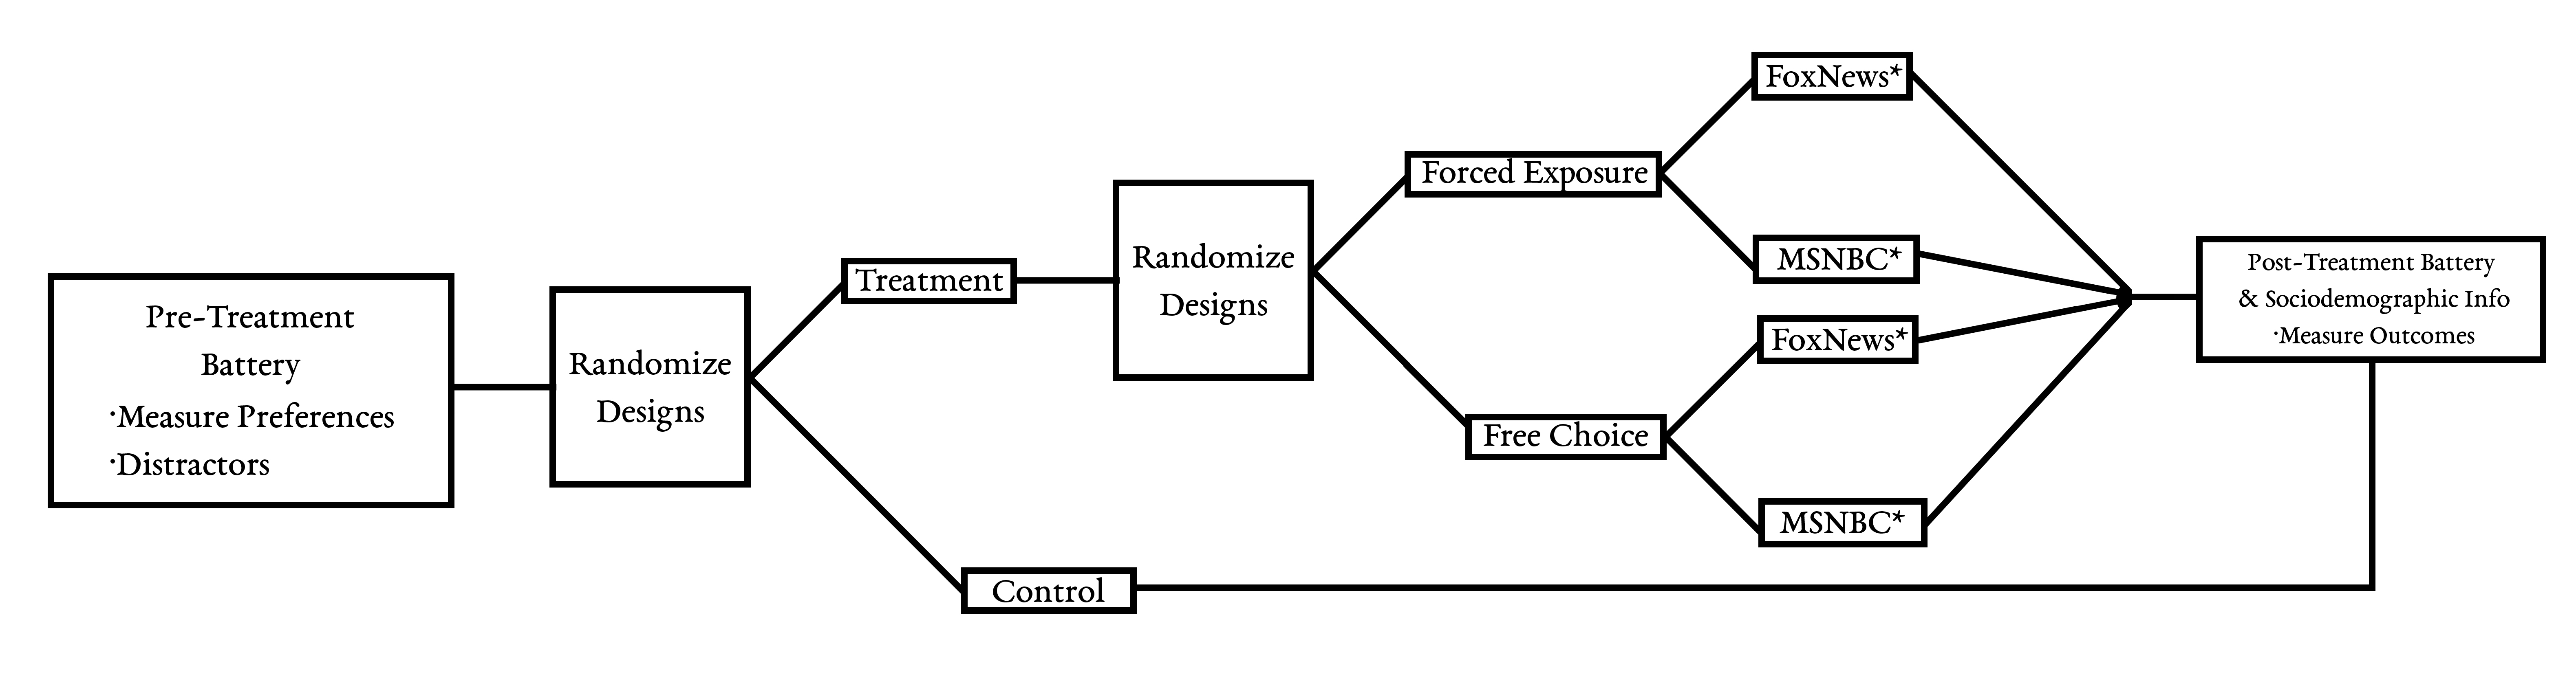
\includegraphics{../prereg/Lab-Graphic.jpg}
\caption{\label{fig:flow}Survey flow and overview of the experimental
design. See Appendix D for the complete questionnaire.}
\end{figure}

\doublespacing

\noindent Depending on their preference (in the free choice condition)
or random assignment (in the forced exposure condition), participants
are then shown one of the tweets displayed in Figure \ref{fig:tweets},
which links to a news story focusing on immigrant-owned businesses in
the U.S. Importantly, both tweets contain exactly the same information,
so regardless of which news organization participants chose (or were
assigned to), the information itself is held constant. After viewing one
of the tweets, participants are asked to read the corresponding article.
As before, the content of the news article is held constant across
sources in either condition.\footnote{See Appendix D for the full news
  article. Using the same content across news networks may cause some
  participants to be skeptical of the source attribution in their
  respective condition (e.g., how plausible is it that Fox News would
  publish a positive article on immigration?). Keeping this in issue in
  mind, we composed the content such that it emphasized a pro-business
  perspective highlighting the economic benefits of immigration through
  entrepreneurship, which was intended to appear as realistic business
  reporting that could conceivably be published by either network. While
  we didn't ask respondents directly whether they consider the article
  to be authentic (in order to avoid related priming effects), we asked
  them to evaluate the news article on various dimensions such as
  ``accurate vs.~inaccurate'' or ``good vs.~bad.'' The response patterns
  conditional on the article's source and the participants' media
  preference suggest that they considered the source attribution to be
  believable (see Appendix A.IV for details). We thank an anonymous
  reviewer for suggesting these additional analyses.}

\singlespace

\begin{figure}
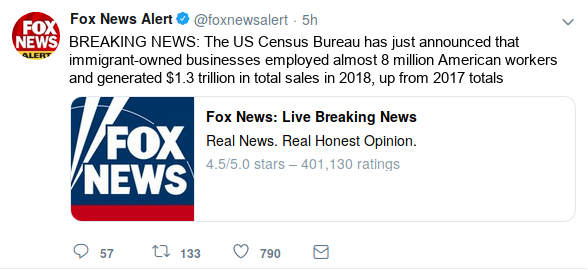
\includegraphics[width=0.5\linewidth]{../material/tweets/fox_popular} 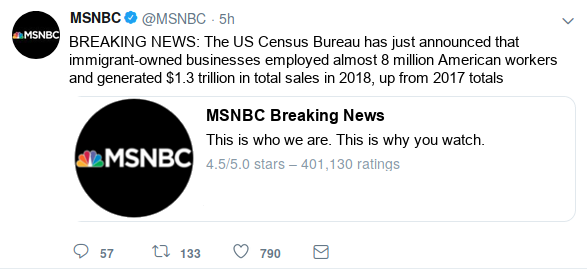
\includegraphics[width=0.5\linewidth]{../material/tweets/msnbc_popular} \caption{\label{fig:tweets}Information treatment on the size of immigrant-owned businesses in the U.S. from two different sources (Fox News or MSNBC). Participants only view one of the tweets.}\label{fig:fig_tweets}
\end{figure}

\doublespace

\noindent Compared to previous implementations of the PICA framework
where the content was not held constant across sources (De
Benedictis-Kessner et al. 2019; Knox et al. 2019), our design allows us
to directly compare the effects of free choice and forced exposure while
ensuring that differences between treatment groups are not the result of
the structure, content, or tone of different stories. Finally,
participants who are randomly assigned to the control group skip the
tweet and article entirely and move directly from the pretreatment
battery to the outcome measures.

\begin{table}[!h]

\caption{\label{tab:tab_outcomes}\label{tab:outcomes}Overview of outcome variables measuring beliefs, interpretation, and opinions related to the economic impact of legal immigration in the U.S.}
\centering
\begin{tabular}[t]{>{\raggedright\arraybackslash}p{4cm}>{\raggedright\arraybackslash}p{6cm}>{\raggedright\arraybackslash}p{5cm}}
\toprule
Belief & Interpretation & Opinion\\
\midrule
Across the United States, how many workers--immigrant and US-born--do you think are employed by immigrant-owned businesses? & On average, would you say that people who come to live here from other countries will take jobs away from people already here or add to the economy by creating additional jobs? & Do you think the number of immigrants from foreign countries who are permitted to come to the United States to live should be [increased/left the same/decreased]\\
 &  & \\
Taking your best guess, what was the total amount of sales revenue of immigrant-owned businesses in the last year? & Most people who come to live in the U.S. work and pay taxes. They also use health and social services. On balance, do you think people who come here take out more than they put in or put in more than they take out? & \\
\bottomrule
\end{tabular}
\end{table}

For our analysis, we consider five different outcomes that correspond to
beliefs, interpretations, and opinions related to the economic impact of
legal immigration. The full question overview is displayed in Table
\ref{tab:outcomes}. Two items targeting factual \emph{beliefs} directly
ask for statistics regarding the number of workers employed by
immigrant-owned businesses as well as the total amount of sales revenue
of immigrant-owned businesses. Both questions offer five response
options, (one of which is accurate) and the correct information is
mentioned in the tweet as well as the news article. In order to measure
\emph{interpretations} consistent with the theoretical conceptualization
discussed above, we asked respondents two additional questions about
whether they believe that immigrants add to the economy by creating
additional jobs and whether they contribute more by paying taxes than
they take out by using health and social services. Lastly, we measure
\emph{opinions} by asking for the participants' overall preference
regarding the number of immigrants who should be allowed to move to and
live in the United States. Together, these outcome measures allow for a
more fine-grained differentiation of possible types of (incomplete)
updating than previous studies on the effectiveness of misinformation
corrections. In the following section, we are going to leverage this
differentiation to examine how the ability to choose information sources
moderates their impact on beliefs, interpretations, and opinions.

Our analytical strategy to identify the news article's impact on each of
these outcome measures is based on between-subject comparisons across
treatment conditions. As such, we are relying on the fact that most
people tend to underestimate the beneficial economic impact of
immigration and are therefore likely to hold incorrect factual beliefs
prior to reading the article---a common approach in previous studies
exploring the effect of corrective information on attitudes about
immigration (e.g., Hopkins, Sides, and Citrin 2019).\footnote{In the
  control condition (i.e., without exposure to corrective information),
  only about 5\% of respondents answered both factual questions about
  the economic impact of legal immigration correctly.} Our reliance on
between-subject comparisons is furthermore in accordance with prior
implementations of the PICA design (e.g., De Benedictis-Kessner et al.
2019), due to the fact that genuine genuine within-subject comparisons
would require the same set of attitude measures before and after
exposure to the article. However, repeating the same questions on the
same topic as the article may jeopardize the information treatment
itself, since participants may then doubt that they are given a
``random'' news article as described in the survey instructions.

In order to increase the precision of our estimated treatment effects,
we follow recent recommendations by Clifford, Sheagley, and Piston
(2021) and incorporate two pretreatment measures capturing general
immigration attitudes that should be highly predictive of our outcome
measures.\footnote{See Appendix D.I for full question wording.} These
measures were embedded in a set of distractor items to disguise their
connection to the news article. In particular, we asked respondents to
rank the importance of five different problems facing the country---one
of which being immigration. Additionally, we included a battery of
questions on explicit social stereotypes---one of which focusing on
whether participants viewed Hispanic-Americans as ``hardworking'' or
``lazy.'' Again, these items were embedded in a broader set of questions
covering stereotypes about different occupational groups and age groups.
Thus, while we are employing between-subjects comparisons consistent
with previous studies in this area, we incorporate elements of a ``quasi
pretest-posttest design'' (Clifford, Sheagley, and Piston 2021) by
controlling for pretreatment covariates that are highly predictive of
our outcome measures---thereby improving precision and controlling for
potential imbalance in observed confounders.

\hypertarget{results}{%
\section{Results}\label{results}}

We preregistered our study on
\censor{EGAP (Registration ID: 20191119AC)} prior to data
collection.\footnote{A shortened and de-identified version of the
  registration and pre-analysis plan is included in Appendix E.} The
survey was fielded on Amazon's Mechanical Turk (MTurk) in December 2019
with a sample of 600 respondents. We provide an overview of our sample
demographics across treatment conditions as well as balance checks in
Appendix A. In general, respondents on MTurk tend to be younger, more
liberal, and more educated than the average U.S. population (Huff and
Tingley 2015). However, while MTurk samples are not representative of
the broader U.S. population, they are more diverse than other
convenience samples such as college students (Berinsky, Huber, and Lenz
2012) and have been shown to be suitable for survey experiments
(Krupnikov and Levine 2014). Indeed, extensive research has demonstrated
that results derived from online convenience samples are similar to
those obtained from national samples (Clifford, Jewell, and Waggoner
2015; Coppock 2019; Coppock and McClellan 2019).

Recently, however, there has been concern about declining data quality
on MTurk---particularly due to the use of virtual private networks
(VPNs) to circumvent location restrictions implemented in surveys
designed for U.S. participants only (Kennedy et al. 2020). Since these
fraudulent respondents tend to provide substantially lower-quality
responses, we followed current best practices by implementing an
automatic script in our survey that identifies and screens out bots and
users who mask their true location via VPNs (Winter et al. 2019;
Waggoner, Kennedy, and Clifford 2019). In addition, we included
attention checks at the end of our survey to make sure that respondents
read the material carefully. Only a small proportion failed our
attention checks (less than 10\%), but we refrained from dropping these
respondents in order to avoid post-treatment bias (Aronow, Baron, and
Pinson 2019). That said, the substantive results presented in the
following remain unchanged when excluding non-attentive respondents.

\hypertarget{free-choice-enables-opinion-change}{%
\subsection{Free Choice Enables Opinion
Change}\label{free-choice-enables-opinion-change}}

As a first step, we examine average treatment effects of the forced
exposure and free choice conditions relative to the control group that
did not have access to the tweet or news article. For each of the five
outcome measures, we estimate a linear regression with two treatment
indicators as main independent variables (the control condition is the
reference category) while controlling for a set of pretreatment
attitudes and sociodemographic characteristics to increase statistical
power (c.f., Bowers 2011; Clifford, Sheagley, and Piston 2021). Figure
\ref{fig:m1} displays the estimated treatment effects based on these
models.\footnote{Full regression tables including controls can be found
  in Appendix C.} Since the measures of factual beliefs are dichotomous
(correct vs.~incorrect), the first set of coefficients examining belief
change can be interpreted as linear probability models (LPM), whereas
the remaining coefficients can be interpreted as average treatment
effects where the (quasi-)continuous outcome variable has been rescaled
to range from zero to one.

We use the LPM instead of a logit or probit model to facilitate easier
comparisons across the range of outcomes considered in our analysis. The
linear probability model is particularly useful when analyzing
experimental data with dichotomous outcomes, since parameter estimates
can be directly interpreted as average marginal treatment effects on the
probability scale (see Angrist and Pischke 2008; Greene 2008 for
details).\footnote{The main disadvantage of the LPM is that it fails to
  capture the inherently non-linear relationship between binary outcomes
  and continuous predictors, which may ultimately result in predicted
  probabilities that are less than 0 or greater than 1. However, failing
  to account for the non-linear functional form is less of an issue when
  estimating the effect of \emph{dichotomous} treatment indicators,
  which is further illustrated by the fact that our linear probability
  models produce less than 2\% out-of-bounds predictions across all
  specifications discussed below. Notwithstanding, we replicate
  equivalent results using logistic regression in Appendix B.III.}
Furthermore, since the remaining non-dichotomous outcomes variables all
range between zero and one, we can easily evaluate and compare treatment
effects across models.

\singlespace

\begin{figure}
\centering
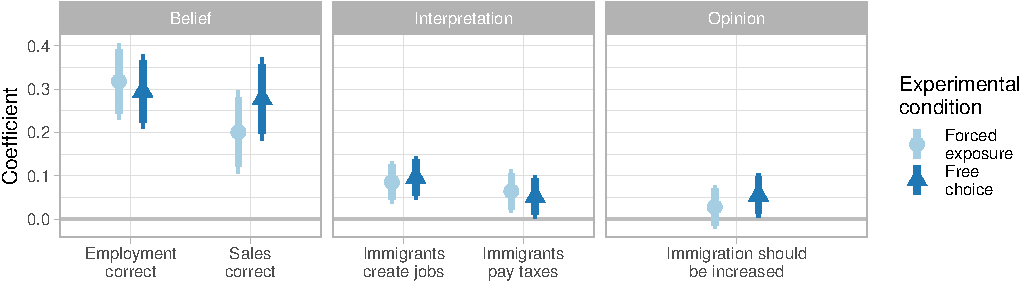
\includegraphics{ReliableSources_files/figure-latex/m1-1.pdf}
\caption{\label{fig:m1}Treatment effects of forced exposure and free
choice manipulation (vs.~control). Coefficients are based on linear
regression models controlling for pretreatment immigration attitudes,
political predispositions, and sociodemographics. Positive coefficients
indicate larger probability of correct responses (Belief) or more
liberal immigration attitudes (Interpretation \& Opinion). 90\% (thick
line) and 95\% (thin line) confidence intervals based on robust standard
errors. Appendix C displays full model results.}
\end{figure}

\doublespace

\noindent Focusing first on the effect of corrective information on
factual beliefs, the proportion of correct responses regarding the
employment and total value of sales by immigrant-owned businesses is
about 20 to 30 percentage points higher among participants who read the
tweet and news story than among participants in the control condition.
This is a substantively large effect and it is illustrative of the fact
that participants systematically underestimated the economic
contributions of immigrant-owned business if they were not given any
additional information.

Turning to the effect of corrective information on interpretations, we
find smaller, but still statistically significant treatment effects.
After reading the tweet and news story, participants provided a more
favorable assessment regarding the number of jobs created by immigrants
as well as the relative size of their tax contributions. As before, this
effect is significant for both the forced exposure and the free choice
conditions.

Lastly, the treatment effect of forced exposure to corrective
information largely diminishes when focusing on opinion change as the
outcome of interest, which is consistent with previous experimental
evidence (e.g., Hopkins, Sides, and Citrin 2019). In contrast, however,
we do observe a small but statistically significant increase in general
support for legal immigration among participants in the free choice
condition compared to the control group. The finding that people's
opinions toward legal immigration only change in response to
\emph{voluntary} exposure to corrective information is consistent with
the argument that freedom of choice reduces negative affect and
counter-arguing towards the source (Stroud et al. 2019). Before drawing
any definite conclusions regarding this proposed mechanism, however, we
need to explore the impact of media preferences and source consistency
in this context. This will be the focus of the subsequent section.

Summarizing our results thus far, the finding that estimated treatment
effects are smaller for interpretations and opinions than for beliefs
strongly supports Hypothesis 1. In addition, differences between the
forced exposure and free choice conditions appear fairly limited across
outcomes. Updating beliefs and interpretations as a response to
misinformation corrections is relatively common and independent of how
people gain access to them. Only if people are allowed to choose their
information source, however, do we observe that they change their
opinions about the issue. While this is at least suggestive evidence
that discretion over media diets is a potentially important factor
facilitating opinion change, it should be noted that the difference
between both treatment effects themselves is not statistically
significant (see also Gelman and Stern 2006). Overall, these results
lend at least some support to Hypothesis 2. Next, we are going to
incorporate people's preferences over specific media sources in the
analysis to further corroborate our findings.

\hypertarget{opinion-change-is-driven-by-voluntary-exposure-to-inconsistent-sources}{%
\subsection{Opinion Change is Driven by Voluntary Exposure to
Inconsistent
Sources}\label{opinion-change-is-driven-by-voluntary-exposure-to-inconsistent-sources}}

At the beginning of our survey experiment, we included a battery of
questions regarding people's usual media diet. Based on these items, we
can distinguish whether participants in the treatment conditions were
exposed to an information source that is consistent or inconsistent with
their usual media preferences (if they usually prefer to watch more Fox
News than MSNBC and vice versa), or if the information source is neutral
(if they prefer neither Fox News nor MSNBC as part of their usual media
diet). Figure \ref{fig:m2} repeats the previous analysis examining
treatment effects on beliefs, interpretations, and opinions---but now
differentiating participants in the forced exposure and free choice
conditions by source consistency.

\singlespace

\begin{figure}
\centering
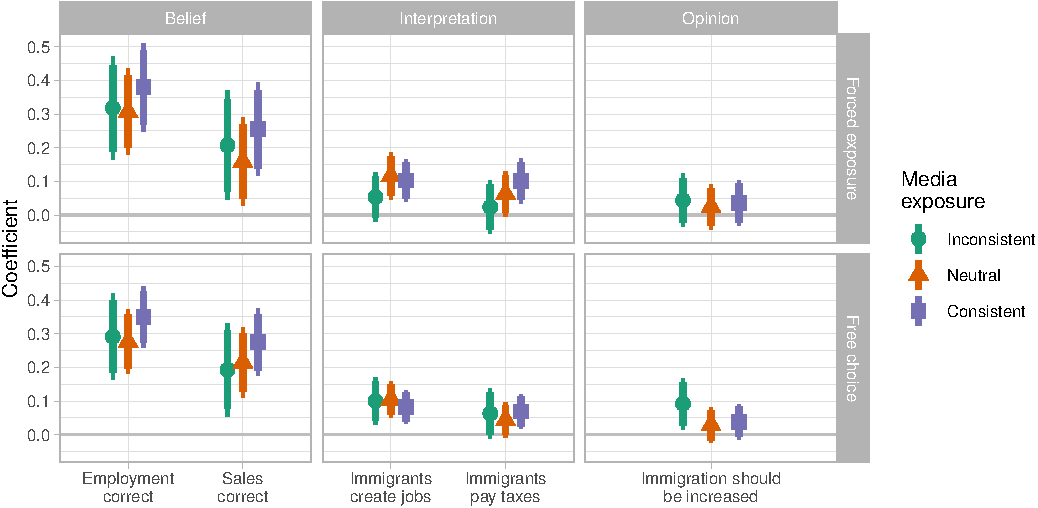
\includegraphics{ReliableSources_files/figure-latex/m2-1.pdf}
\caption{\label{fig:m2}Treatment effects of forced exposure and free
choice manipulation (vs.~control) conditional on consistency between
media preference and information source. Coefficients are based on
linear regression models controlling for pretreatment immigration
attitudes, political predispositions, and sociodemographics. Positive
coefficients indicate larger probability of correct responses (Belief)
or more liberal immigration attitudes (Interpretation \& Opinion). 95\%
(thin line) and 90\% (thick line) confidence intervals based on robust
standard errors. Appendix C displays full model results.}
\end{figure}

\doublespace

\noindent Focusing first on beliefs and interpretations as outcomes, we
observe slightly larger treatment effects for participants who were
exposed to an information source that is consistent with their usual
media diet---a pattern that holds in the forced exposure as well as the
free choice condition. In fact, in three out of four analyses, the
information treatment had no statistically significant effect on
people's interpretations regarding the economic benefits of legal
immigration if it came from an inconsistent source, whereas exposure to
a consistent source was always associated with more favorable
interpretations. This result largely supports our third hypothesis that
corrections will have stronger effects if the information source is
consistent with respondents' media preferences.

Interestingly, this pattern is reversed for opinion change as a response
to the news story. To the extent that the positive treatment effect of
the free choice condition on opinions reported in Figure \ref{fig:m1} is
solely driven by people's tendency to seek out consistent sources, we
would expect a similar effect when focusing on forced exposure to
consistent sources. This is not the case. Regardless of whether
participants were given a news source that is consistent with their
usual media diet, the information treatment in the forced exposure
condition had no effect on subsequent opinions regarding the desired
level of immigration in the U.S. In the free choice condition, on the
other hand, we do find evidence for opinion change compared to control
condition. Surprisingly, however, it is exposure to \emph{inconsistent}
sources in the free choice condition that ultimately results in
significant opinion change.

\singlespace

\begin{figure}
\centering
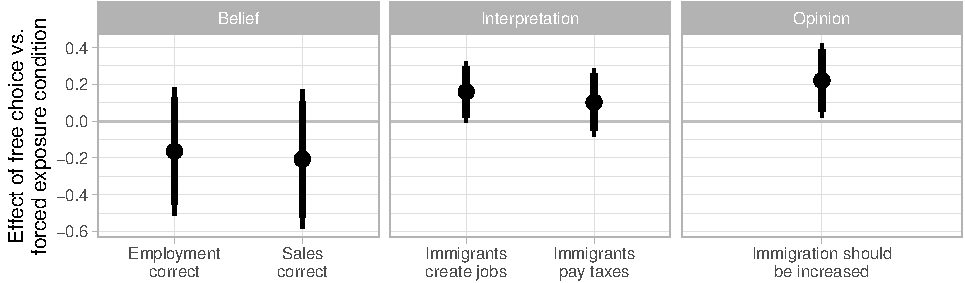
\includegraphics{ReliableSources_files/figure-latex/m4-1.pdf}
\caption{\label{fig:m4}Difference in treatment effects of free choice
manipulation (vs.~forced exposure) conditional on exposure to
information source that is inconsistent with media preference.
Coefficients are based on linear regression models controlling for
pretreatment immigration attitudes, political predispositions, and
sociodemographics. Positive coefficients indicate larger treatment
effect for voluntary (vs.~involuntary) exposure to inconsistent source.
95\% (thin line) and 90\% (thick line) confidence intervals based on
robust standard errors. Appendix C displays full model results.}
\end{figure}

\doublespace

\noindent To further corroborate this finding, we now directly compare
the effect of voluntary and involuntary exposure to inconsistent
sources. Specifically, we reduce the sample to include only participants
who were exposed to a news source that was inconsistent with their usual
media diet. We then run regressions using the same specifications as
before, now only including a single treatment indicator for the free
choice condition. Note that since this specification omits the control
group and instead uses forced exposure to inconsistent sources as the
reference category, the coefficients can be directly interpreted as the
differences in treatment effects between the free choice and forced
exposure condition. The results are displayed in Figure \ref{fig:m4}.

Conditional on exposure to an inconsistent source, there are no clear
differences in treatment effects on beliefs and related interpretations.
However, participants who were exposed to inconsistent sources in the
free choice condition reported more favorable opinions towards
immigrants than participants who were exposed to inconsistent sources in
the forced exposure condition. This finding is quite remarkable
considering the fact that regardless of the news organization, the
actual content of the tweet and article was constant across all
treatments.

In sum, changing people's minds by giving them free choice over their
media diet is not driven by the ability to choose consistent news
sources. On the contrary, only participants who voluntarily accessed
information from an inconsistent source reported significantly different
opinions than the control group. In the next section, we explore
potential explanations for this striking result.

\hypertarget{the-role-of-self-selection-pretreatment-attitudes-and-ambivalence6}{%
\subsection[The Role of Self-Selection, Pretreatment Attitudes, and
Ambivalence]{\texorpdfstring{The Role of Self-Selection, Pretreatment
Attitudes, and
Ambivalence\footnote{The analyses in this section were not preregistered
  and should therefore be considered exploratory.}}{The Role of Self-Selection, Pretreatment Attitudes, and Ambivalence}}\label{the-role-of-self-selection-pretreatment-attitudes-and-ambivalence6}}

When evaluating differences between voluntary and involuntary exposure
to inconsistent sources, we have to keep in mind that conditioning on
source selection in the free choice condition makes it challenging to
provide a clear causal interpretation. To the extent that some people
are systematically more likely to self-select inconsistent exposure, any
resulting imbalance in pretreatment confounders could jeopardize our
inferences regarding the causal effect of corrective
information.\footnote{See Appendix A.II for an overview of respondents'
  media preferences and source consistency across treatment groups, and
  Appendix and A.III for the determinants of choosing Fox News in the
  free choice condition.} Given our between-subjects design, the crucial
question then becomes whether people who are willing to access
inconsistent sources (a) hold systematically different pretreatment
attitudes or (b) respond differently to the treatment itself?

Thus, the most obvious alternative explanation for diverging opinions in
response to voluntary and involuntary exposure to inconsistent sources
is that both treatment groups may simply have different attitudes to
begin with. However, all our analyses discussed hitherto include
statistical controls for pretreatment immigration attitudes, racial
stereotypes, ideology, partisanship, and basic
sociodemographics---rendering potential confounding due to these
(observed) characteristics unlikely. A related concern may be that
inconsistent sources are more likely to be selected by people who prefer
MSNBC rather than Fox (or vice versa). First, such imbalances would be
problematic since media preferences are correlated with political
predispositions (e.g., Stroud 2011). Second, since we hold the article
content constant across outlets, it may be viewed as less coherent with
the usual narrative of Fox News and thereby influence people's
receptivity. These concerns are alleviated by the fact that exposure to
Fox News and MSNBC is split evenly among participants who selected
inconsistent sources, which implies that the ratio of both outlets is
balanced between the free-choice and forced exposure condition.
Furthermore, additional analyses in Appendix B.I suggest that there are
no differences in average choice-specific treatment effects
(ACTEs)\footnote{See Knox et al. (2019) for details on estimating ACTEs
  in PICA designs.} between people who prefer Fox or MSNBC and that---if
anything---people who usually prefer MSNBC appear more biased against
Fox News than people who usually prefer Fox News are biased against
MSNBC.

Although the results are therefore unlikely to be driven by pretreatment
differences in support for immigration or other predispositions, there
might still be systematic discrepancies in the nature of people's
attitudes. Specifically, people who select inconsistent sources may be
more ambivalent about immigration and therefore more open to opinion
change (e.g., Lavine, Johnston, and Steenbergen 2012). While our
questionnaire did not include a pretreatment measure of ambivalence, we
can assess the plausibility of this alternative explanation by
leveraging open-ended responses included at the end of our survey. After
answering both questions measuring people's \emph{interpretations}
regarding the economic contributions of immigrants (by paying taxes and
creating jobs), participants were asked to explain their previous
assessment in a few sentences.\footnote{See Appendix D.III for full
  question wording.} To the extent that there are differences in
pretreatment ambivalence between voluntary and involuntary exposure to
inconsistent information, these should also manifest in open-ended
responses after reviewing the article. We measure ambivalence using the
well-established LIWC dictionary (Pennebaker et al. 2015), which
includes markers for tentative language (e.g., maybe, perhaps, guess)
that indicate uncertainty about a topic (Tausczik and Pennebaker 2010).
The results are displayed in Figure \ref{fig:m5}.

\singlespace

\begin{figure}
\centering
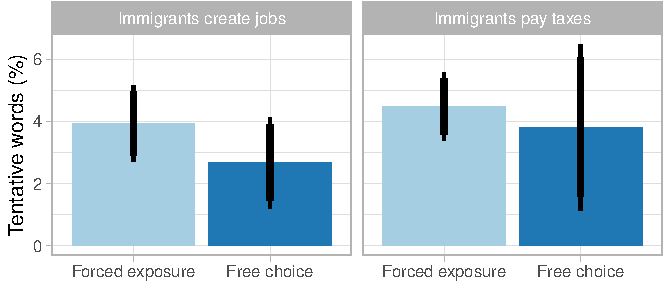
\includegraphics{ReliableSources_files/figure-latex/m5-1.pdf}
\caption{\label{fig:m5}Difference in tentative language in open-ended
responses of respondents who were exposed to inconsistent information in
the free choice and forced exposure condition. Tentative words based on
LIWC dictionary, including 95\% (thin line) and 90\% (thick line)
confidence intervals.}
\end{figure}

\doublespace

\noindent Focusing only on respondents who were exposed to an outlet
that was inconsistent with their media preference, there are no
significant differences in the percentage of tentative words in
open-ended responses between the forced exposure and free choice
conditions. If anything, participants appear less ambivalent after
voluntary exposure to an inconsistent source than after involuntary
exposure to an inconsistent source. In the context of our analyses, this
null finding (i.e., the absence of differences in post-treatment
ambivalence) strongly suggests the absence of pretreatment differences
in ambivalence, unless we are willing to assume that there are
heterogeneous treatment effects that perfectly cancel out prior
differences in ambivalence. We replicate the same result using an
alternative measurement approach in Appendix B.II. Overall, it is
therefore unlikely that the observed opinion change in response to
voluntary exposure to inconsistent sources can be explained by attitude
ambivalence prior to receiving the treatment.

In sum, while we cannot fully rule out the possibility that people who
self-select inconsistent sources have substantively different (or more
ambivalent) pretreatment attitudes, it appears more plausible that the
patterns reflect differences in people's receptiveness to corrective
information. From a theoretical perspective, this could be explained by
the fact that giving people freedom of choice decreases reactance and
cognitive dissonance and thereby reduces counter-arguing (Stroud et al.
2019). Given that we do not observe opinion change in response to
voluntary exposure to \emph{consistent} information, however, this
explanation alone appears to be incomplete as well. In addition to
freedom of choice, what is needed for corrective information to be
effective is that people are sufficiently motivated to seek out
alternative viewpoints in the first place.

\hypertarget{discussion-and-conclusion}{%
\section{Discussion and Conclusion}\label{discussion-and-conclusion}}

The apparent pervasiveness of misinformation across a wide range of
political issues is exacerbated by an increasingly polarized media
environment where people have unprecedented access to a wide variety of
media sources. When it comes to the effectiveness of corrective
interventions, revising people's factual \emph{beliefs} is relatively
easy, while changing their underlying \emph{opinions} is hard. Yet,
previous research in this context neglected the role of selective
exposure and endogenous information search as moderating the potential
attitudinal impact of corrective information. Our study fills this gap
in the literature by employing an experimental design that allows a
subset of participants to choose their information source. Holding the
actual content constant, we find that the ability to choose news sources
facilitates opinion change. However, the effect of people's discretion
over their information intake is not driven by their tendency to access
sources that are consistent with their usual media diet. Rather, it is
the voluntary exposure to inconsistent sources that results in opinion
change.

Of course, our findings are not without limitations. Most importantly,
it is worth emphasizing again that conditioning on (in)consistent
exposure in the free choice condition makes it difficult to provide a
clear causal interpretation of the effects. While our analyses control
for political predispositions and pretreatment immigration attitudes, we
cannot fully rule out the possibility that people who self-selected into
exposure to an inconsistent source had substantively different or more
ambivalent attitudes before receiving the treatment. However, given our
exploratory examination of self-selection and ambivalence, it seems more
likely that people who self-select inconsistent sources are ultimately
more receptive to corrective information (rather than holding different
baseline attitudes or being ambivalent). In addition, the fact that we
do observe significant treatment effects for the free choice condition
(and not for the forced exposure condition) across the entire sample
further alleviates concerns about pretreatment confounding, since this
relationship cannot be explained by self-selection alone.
Notwithstanding, additional research is needed to further corroborate
this conclusion by examining opinion change in response to
misinformation corrections in the context of a within-subjects design.

Overall, our findings indicate that discretion over information sources
facilitates opinion change in response to corrective
information---particularly when people are willing to consider
alternative views. Future studies on misinformation should therefore
incorporate endogenous information search as a crucial component of
their experimental designs, and, from a theoretical perspective,
re-orient their attention to people's underlying motivations to seek out
different sources (e.g., Kunda 1990). In terms of policy implications,
our research strongly suggests that encouraging people to voluntarily
access alternative media outlets may be a more effective strategy to
combat misinformation than providing fact-checks alone.

\clearpage
\parskip=10pt
\singlespace

\hypertarget{bibliography}{%
\section*{References}\label{bibliography}}
\addcontentsline{toc}{section}{References}

\hypertarget{refs}{}
\begin{CSLReferences}{1}{0}
\leavevmode\hypertarget{ref-alesina2019immigration}{}%
Alesina, Alberto, Armando Miano, and Stefanie Stantcheva. 2019.
{``Immigration and Redistribution.''} National Bureau of Economic
Research.

\leavevmode\hypertarget{ref-althaus1998information}{}%
Althaus, Scott L. 1998. {``Information Effects in Collective
Preferences.''} \emph{American Political Science Review} 92 (3):
545--58.

\leavevmode\hypertarget{ref-angrist2008mostly}{}%
Angrist, Joshua D, and Jörn-Steffen Pischke. 2008. \emph{Mostly Harmless
Econometrics: An Empiricist's Companion}. Princeton University Press.

\leavevmode\hypertarget{ref-arceneaux2012polarized}{}%
Arceneaux, Kevin, Martin Johnson, and Chad Murphy. 2012. {``Polarized
Political Communication, Oppositional Media Hostility, and Selective
Exposure.''} \emph{The Journal of Politics} 74 (01): 174--86.

\leavevmode\hypertarget{ref-aronow2019note}{}%
Aronow, Peter M, Jonathon Baron, and Lauren Pinson. 2019. {``A Note on
Dropping Experimental Subjects Who Fail a Manipulation Check.''}
\emph{Political Analysis} 27 (4): 572--89.

\leavevmode\hypertarget{ref-bartels1996uninformed}{}%
Bartels, Larry M. 1996. {``Uninformed Votes: Information Effects in
Presidential Elections.''} \emph{American Journal of Political Science}
40 (1): 194--230.

\leavevmode\hypertarget{ref-berinsky2017rumors}{}%
Berinsky, Adam J. 2017. {``Rumors and Health Care Reform: Experiments in
Political Misinformation.''} \emph{British Journal of Political Science}
47 (2): 241--62.

\leavevmode\hypertarget{ref-berinsky2012evaluating}{}%
Berinsky, Adam J, Gregory A Huber, and Gabriel S Lenz. 2012.
{``Evaluating Online Labor Markets for Experimental Research:
Amazon.com's Mechanical Turk.''} \emph{Political Analysis} 20 (3):
351--68.

\leavevmode\hypertarget{ref-bowers2011making}{}%
Bowers, Jake. 2011. {``Making Effects Manifest in Randomized
Experiments.''} In \emph{Cambridge Handbook of Experimental Political
Science}. Cambridge University Press.

\leavevmode\hypertarget{ref-clifford2015samples}{}%
Clifford, Scott, Ryan M Jewell, and Philip D Waggoner. 2015. {``Are
Samples Drawn from Mechanical Turk Valid for Research on Political
Ideology?''} \emph{Research \& Politics} 2 (4): 2053168015622072.

\leavevmode\hypertarget{ref-clifford2021increasing}{}%
Clifford, Scott, Geoffrey Sheagley, and Spencer Piston. 2021.
{``Increasing Precision Without Altering Treatment Effects: Repeated
Measures Designs in Survey Experiments.''} \emph{American Political
Science Review}, 1--18.

\leavevmode\hypertarget{ref-coppock2019generalizing}{}%
Coppock, Alexander. 2019. {``Generalizing from Survey Experiments
Conducted on Mechanical Turk: A Replication Approach.''} \emph{Political
Science Research and Methods} 7 (3): 613--28.

\leavevmode\hypertarget{ref-coppock2019validating}{}%
Coppock, Alexander, and Oliver A McClellan. 2019. {``Validating the
Demographic, Political, Psychological, and Experimental Results Obtained
from a New Source of Online Survey Respondents.''} \emph{Research \&
Politics} 6 (1): 2053168018822174.

\leavevmode\hypertarget{ref-benedictis2019persuading}{}%
De Benedictis-Kessner, Justin, Matthew A Baum, Adam J Berinsky, and
Teppei Yamamoto. 2019. {``Persuading the Enemy: Estimating the
Persuasive Effects of Partisan Media with the Preference-Incorporating
Choice and Assignment Design.''} \emph{American Political Science
Review} 113 (4): 902--16.

\leavevmode\hypertarget{ref-flynn2017nature}{}%
Flynn, DJ, Brendan Nyhan, and Jason Reifler. 2017. {``The Nature and
Origins of Misperceptions: Understanding False and Unsupported Beliefs
about Politics.''} \emph{Political Psychology} 38: 127--50.

\leavevmode\hypertarget{ref-gaines2007same}{}%
Gaines, Brian J, James H Kuklinski, Paul J Quirk, Buddy Peyton, and Jay
Verkuilen. 2007. {``Same Facts, Different Interpretations: Partisan
Motivation and Opinion on Iraq.''} \emph{Journal of Politics} 69 (4):
957--74.

\leavevmode\hypertarget{ref-gelman2006difference}{}%
Gelman, Andrew, and Hal Stern. 2006. {``The Difference Between
{`Significant'} and {`Not Significant'} Is Not Itself Statistically
Significant.''} \emph{The American Statistician} 60 (4): 328--31.

\leavevmode\hypertarget{ref-greene2008econometric}{}%
Greene, William H. 2008. \emph{Econometric Analysis}. Granite Hill
Publishers.

\leavevmode\hypertarget{ref-guess2020exposure}{}%
Guess, Andrew M, Brendan Nyhan, and Jason Reifler. 2020. {``Exposure to
Untrustworthy Websites in the 2016 US Election.''} \emph{Nature Human
Behaviour}.

\leavevmode\hypertarget{ref-guillory2013correcting}{}%
Guillory, Jimmeka J, and Lisa Geraci. 2013. {``Correcting Erroneous
Inferences in Memory: The Role of Source Credibility.''} \emph{Journal
of Applied Research in Memory and Cognition} 2 (4): 201--9.

\leavevmode\hypertarget{ref-hainmueller2014public}{}%
Hainmueller, Jens, and Daniel J Hopkins. 2014. {``Public Attitudes
Toward Immigration.''} \emph{Annual Review of Political Science} 17.

\leavevmode\hypertarget{ref-hopkins2019muted}{}%
Hopkins, Daniel J, John Sides, and Jack Citrin. 2019. {``The Muted
Consequences of Correct Information about Immigration.''} \emph{The
Journal of Politics} 81 (1): 315--20.

\leavevmode\hypertarget{ref-huff2015these}{}%
Huff, Connor, and Dustin Tingley. 2015. {``{`Who Are These People?'}
Evaluating the Demographic Characteristics and Political Preferences of
MTurk Survey Respondents.''} \emph{Research \& Politics} 2 (3):
2053168015604648.

\leavevmode\hypertarget{ref-iyengar2009red}{}%
Iyengar, Shanto, and Kyu S Hahn. 2009. {``Red Media, Blue Media:
Evidence of Ideological Selectivity in Media Use.''} \emph{Journal of
Communication} 59 (1): 19--39.

\leavevmode\hypertarget{ref-kalla2020reducing}{}%
Kalla, Joshua, and David Broockman. 2020. {``Reducing Exclusionary
Attitudes Through Interpersonal Conversation: Evidence from Three Field
Experiments.''} \emph{American Political Science Review} 114 (2):
410--25.

\leavevmode\hypertarget{ref-kennedy2020shape}{}%
Kennedy, Ryan, Scott Clifford, Tyler Burleigh, Philip D Waggoner, Ryan
Jewell, and Nicholas JG Winter. 2020. {``The Shape of and Solutions to
the MTurk Quality Crisis.''} \emph{Political Science Research and
Methods} 8 (4): 614--29.

\leavevmode\hypertarget{ref-knox2019design}{}%
Knox, Dean, Teppei Yamamoto, Matthew A Baum, and Adam J Berinsky. 2019.
{``Design, Identification, and Sensitivity Analysis for Patient
Preference Trials.''} \emph{Journal of the American Statistical
Association} 114 (528): 1532--46.

\leavevmode\hypertarget{ref-krupnikov2014cross}{}%
Krupnikov, Yanna, and Adam Seth Levine. 2014. {``Cross-Sample
Comparisons and External Validity.''} \emph{Journal of Experimental
Political Science} 1 (01): 59--80.

\leavevmode\hypertarget{ref-kuklinski2000misinformation}{}%
Kuklinski, James H, Paul J Quirk, Jennifer Jerit, David Schwieder, and
Robert F Rich. 2000. {``Misinformation and the Currency of Democratic
Citizenship.''} \emph{Journal of Politics} 62 (3): 790--816.

\leavevmode\hypertarget{ref-kunda1990case}{}%
Kunda, Ziva. 1990. {``The Case for Motivated Reasoning.''}
\emph{Psychological Bulletin} 108 (3): 480--98.

\leavevmode\hypertarget{ref-lavine2012ambivalent}{}%
Lavine, Howard G, Christopher D Johnston, and Marco R Steenbergen. 2012.
\emph{The Ambivalent Partisan: How Critical Loyalty Promotes Democracy}.
Oxford University Press.

\leavevmode\hypertarget{ref-leeper2020raising}{}%
Leeper, Thomas J. 2020. {``Raising the Floor or Closing the Gap? How
Media Choice and Media Content Impact Political Knowledge.''}
\emph{Political Communication}, 1--22.

\leavevmode\hypertarget{ref-nyhan2019taking}{}%
Nyhan, Brendan, Ethan Porter, Jason Reifler, and Thomas J Wood. 2019.
{``Taking Fact-Checks Literally but Not Seriously? The Effects of
Journalistic Fact-Checking on Factual Beliefs and Candidate
Favorability.''} \emph{Political Behavior}, 1--22.

\leavevmode\hypertarget{ref-pennebaker2015development}{}%
Pennebaker, James W, Ryan L Boyd, Kayla Jordan, and Kate Blackburn.
2015. {``The Development and Psychometric Properties of Liwc2015.''}
Unpublished Manuscript.

\leavevmode\hypertarget{ref-redlawsk2010affective}{}%
Redlawsk, David P., Andrew J. W. Civettini, and Karen M. Emmerson. 2010.
{``The Affective Tipping Point: Do Motivated Reasoners Ever 'Get It'.''}
\emph{Political Psychology} 31 (4): 563--93.

\leavevmode\hypertarget{ref-stroud2010polarization}{}%
Stroud, Natalie Jomini. 2010. {``Polarization and Partisan Selective
Exposure.''} \emph{Journal of Communication} 60 (3): 556--76.

\leavevmode\hypertarget{ref-stroud2011niche}{}%
---------. 2011. \emph{Niche News: The Politics of News Choice}. Oxford
University Press.

\leavevmode\hypertarget{ref-stroud2019consequences}{}%
Stroud, Natalie Jomini, Lauren Feldman, Magdalena Wojcieszak, and Bruce
Bimber. 2019. {``The Consequences of Forced Versus Selected Political
Media Exposure.''} \emph{Human Communication Research} 45 (1): 27--51.

\leavevmode\hypertarget{ref-swire2017processing}{}%
Swire, Briony, Adam J Berinsky, Stephan Lewandowsky, and Ullrich KH
Ecker. 2017. {``Processing Political Misinformation: Comprehending the
Trump Phenomenon.''} \emph{Royal Society Open Science} 4 (3): 160802.

\leavevmode\hypertarget{ref-swire2020they}{}%
Swire-Thompson, Briony, Ullrich KH Ecker, Stephan Lewandowsky, and Adam
J Berinsky. 2020. {``They Might Be a Liar but They're My Liar: Source
Evaluation and the Prevalence of Misinformation.''} \emph{Political
Psychology} 41 (1): 21--34.

\leavevmode\hypertarget{ref-Taber2006}{}%
Taber, Charles S., and Milton Lodge. 2006. {``Motivated Skepticism in
the Evaluation of Political Beliefs.''} \emph{American Journal of
Political Science} 50 (3): 755--69.

\leavevmode\hypertarget{ref-tausczik2010psychological}{}%
Tausczik, Yla R, and James W Pennebaker. 2010. {``The Psychological
Meaning of Words: LIWC and Computerized Text Analysis Methods.''}
\emph{Journal of Language and Social Psychology} 29 (1): 24--54.

\leavevmode\hypertarget{ref-waggoner2019detecting}{}%
Waggoner, Philip D, Ryan Kennedy, and Scott Clifford. 2019. {``Detecting
Fraud in Online Surveys by Tracing, Scoring, and Visualizing IP
Addresses.''} \emph{Journal of Open Source Software} 4 (37): 1--5.

\leavevmode\hypertarget{ref-winter2019simplified}{}%
Winter, Nicholas, Tyler Burleigh, Ryan Kennedy, and Scott Clifford.
2019. {``A Simplified Protocol to Screen Out VPS and International
Respondents Using Qualtrics.''} \emph{Available at SSRN 3327274}.

\leavevmode\hypertarget{ref-Wright2020}{}%
Wright, Chrysalis L., Taylor DeFrancesco, Carissa Hamilton, and Lygia
Machado. 2020. {``The Influence of Media Portrayals of Immigration and
Refugees on Consumer Attitudes: A Experimental Design.''} \emph{Howard
Journal of Communications} 31 (4): 388--410.

\end{CSLReferences}

\end{document}
